\documentclass[crop, tikz]{standalone}
\usepackage{tikz}

\usepackage{xcolor}
\definecolor{morange}{RGB}{255,127,14}
\definecolor{mblue}{RGB}{31,119,180}
\definecolor{mred}{RGB}{214,39,40}
\definecolor{mpurple}{RGB}{148,103,189}
\definecolor{mgreen}{RGB}{44,160,44}


\begin{document}

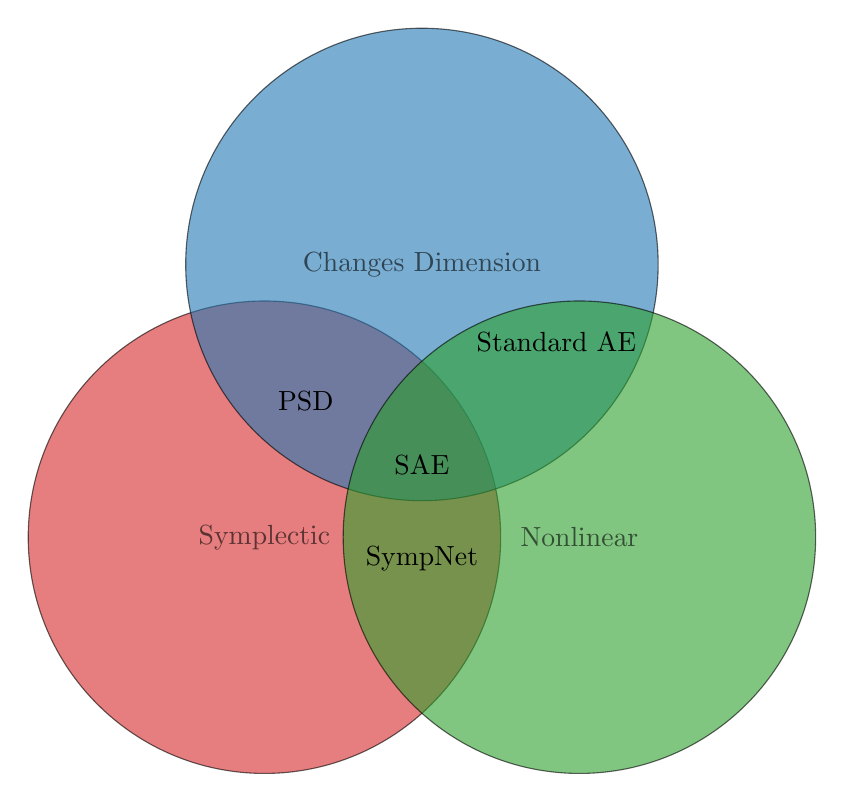
\begin{tikzpicture}
  \tikzset{venn circle/.style={draw,circle,minimum width=6cm,fill=#1,opacity=0.6}}

  \node [venn circle = mred] (A) at (0,0) {Symplectic}; % A
  \node [venn circle = mblue] (B) at (60:4cm) {Changes Dimension}; % B
  \node [venn circle = mgreen] (C) at (0:4cm) {Nonlinear}; % C
  \node[left] at (barycentric cs:A=1/2,B=1/2 ) {PSD}; 
  \node[below] at (barycentric cs:A=1/2,C=1/2 ) {SympNet};   
  \node[right] at (barycentric cs:B=5/7,C=2/7 ) {Standard AE};   
  \node[below] at (barycentric cs:A=1/3,B=1/3,C=1/3 ){SAE};
\end{tikzpicture}  
\end{document}